This question can be a good application of the \textit{secretary problem}. Algorithm is like that:

\begin{itemize}
  \item For $n$, we skip the predefined $k$ elements while keeping the max of the seen elements in the memory.
  \item After $k$ elements, we choose the next larger element than seen max. Here, larger element may not be seen, then we go to the end of the array and choose the last one.
\end{itemize}

Why this algorithm is correct is defined by a simple probability calculation:

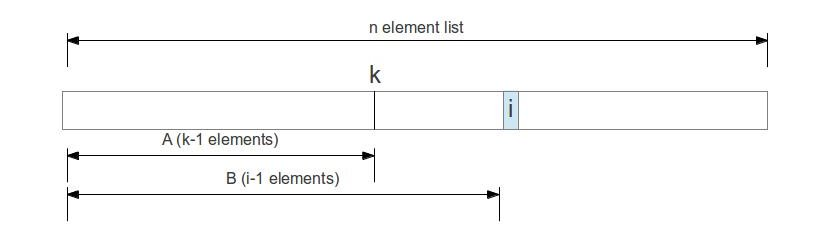
\includegraphics[scale=0.5]{q4}

\begin{equation*}
  \begin{split}
  P(k) &= \sum_{i=1}^{n} P(\text{$i$ selected} | \text{$i$ is the best}) \cdot P(\text{applicant $i$ is the best}) \\
       &= (\sum_{i=1}^{k-1} 0 \cdot \frac{1}{n}) + (\sum_{i=r}^{n} P(
         \text{the best in the first $i-1$} 
         \text{is among the first $k-1$} | \text{$i$ is the best}) \cdot \frac{1}{n}) \\
       &= \sum_{i=k}^{n} \frac{k-1}{i-1} \cdot \frac{1}{n} \\
       &= \frac{k-1}{n} \sum_{i=k}^{n} \frac{1}{i-1} 
  \end{split} 
\end{equation*}

  Since we skip first $k$ elements, the probability of finding max in between them is zero if max is there. However, if max is following the skipped elements, then we can find it with probability $\frac{k-1}{i-1}$ because $i$ is the max and we choose it so max of $i-1$ elements must be in first $k-1$ elements. Otherwise, max would be between $k$ and $i$ and we would choose it, not the actual max.
  
  $k$ can be found iteratively, setting it to 2 going upwards by calculating above result. When we arrive a probability larger than desired probability, algorithm stops. Then, by using found $k$, chooses probable max so skips first $k$ elements but notes down the max of them and after $k$ elements, picks the first element larger than known max.
  
  Here, we provide reference \textit{python} implementation for $k$ finding and testing of found $k$ on all permutations:

\lstinputlisting[language=Python]{q4.py}
